\documentclass[a4paper]{article}

\addtolength{\hoffset}{-2.25cm}
\addtolength{\textwidth}{4.5cm}
\addtolength{\voffset}{-3.25cm}
\addtolength{\textheight}{5cm}
\setlength{\parskip}{0pt}
\setlength{\parindent}{0in}

%----------------------------------------------------------------------------------------
%	PACKAGES AND OTHER DOCUMENT CONFIGURATIONS
%----------------------------------------------------------------------------------------

\usepackage{blindtext} % Package to generate dummy text
\usepackage{charter} % Use the Charter font
\usepackage[utf8]{inputenc} % Use UTF-8 encoding
\usepackage{microtype} % Slightly tweak font spacing for aesthetics
\usepackage[english]{babel} % Language hyphenation and typographical rules
\usepackage{amsthm, amsmath, amssymb} % Mathematical typesetting
\usepackage{float} % Improved interface for floating objects
\usepackage[final, colorlinks = true,
            linkcolor = black,
            citecolor = black]{hyperref} % For hyperlinks in the PDF
\usepackage{graphicx, multicol} % Enhanced support for graphics
\usepackage{xcolor} % Driver-independent color extensions
\usepackage{marvosym, wasysym} % More symbols
\usepackage{rotating} % Rotation tools
\usepackage{censor} % Facilities for controlling restricted text
\usepackage{listings} % Environment for non-formatted code, !uses style file!
\usepackage{pseudocode} % Environment for specifying algorithms in a natural way
 % Environment for f-structures, !uses style file!
\usepackage{booktabs} % Enhances quality of tables
\usepackage{tikz-qtree} % Easy tree drawing tool
 % Configuration for b-trees and b+-trees, !uses style file!
\usepackage[backend=biber,style=numeric,
            sorting=nyt]{biblatex} % Complete reimplementation of bibliographic facilities
\addbibresource{ecl.bib}
\usepackage{csquotes} % Context sensitive quotation facilities
\usepackage[yyyymmdd]{datetime} % Uses YEAR-MONTH-DAY format for dates
\renewcommand{\dateseparator}{-} % Sets dateseparator to '-'
\usepackage{fancyhdr} % Headers and footers
\pagestyle{fancy} % All pages have headers and footers
\fancyhead{}\renewcommand{\headrulewidth}{0pt} % Blank out the default header
\fancyfoot[L]{} % Custom footer text
\fancyfoot[C]{} % Custom footer text
\fancyfoot[R]{\thepage} % Custom footer text
\newcommand{\note}[1]{\marginpar{\scriptsize \textcolor{red}{#1}}} % Enables comments in red on margin
\usepackage{mathtools}
\usepackage{amsmath}
\DeclarePairedDelimiter\abs{\lvert}{\rvert}%
\usepackage{cancel}
\usepackage{minted}
\usepackage{float}
\usepackage{caption}
\usepackage{subcaption}
%-------------------------------

%----------------------------------------------------------------------------------------

%-------------------------------
%	ENVIRONMENT SECTION
%-------------------------------
\pagestyle{fancy}
\usepackage{mdframed}

\usepackage[sfdefault]{FiraSans} %% option 'sfdefault' activates Fira Sans as the default text font
\usepackage[T1]{fontenc}
\renewcommand*\oldstylenums[1]{{\firaoldstyle #1}}


% remove numbering from sections
\usepackage{titlesec}
\titleformat{\section}{\normalfont\Large\bfseries}{}{0pt}{}



%-------------------------------------------------------------------------------------------
%	CUSTOM COMMANDS
%-------------------------------
\newcommand{\gaussian}{\frac{1}{\sigma\sqrt{2\pi}}\exp\left(- \frac{(x-\mu)^2}{2\sigma^2}\right)}
\newcommand{\R}{\mathbb R}

\def\inline{\lstinline[basicstyle=\ttfamily,keywordstyle={}]}


\begin{document}


%-------------------------------
%	TITLE SECTION
%-------------------------------

\fancyhead[C]{}
\hrule \medskip % Upper rule
\begin{minipage}{0.295\textwidth}
\raggedright
\footnotesize
Francisco Javier Sáez Maldonado \hfill\\
franciscojavier.saez@estudiante.uam.es
\hfill\\
\end{minipage}
\begin{minipage}{0.4\textwidth}
\centering
\large
Fingerprint Lab Report\\
\normalsize
Deep Learning for Biometric Signal Processing\\
\end{minipage}
\begin{minipage}{0.295\textwidth}
\raggedleft
\today\hfill\\
\end{minipage}
\medskip\hrule

%-------------------------------
%	CONTENTS
%-------------------------------
\section{Exercise 1}
\subsection{ Copy here the two fingerprint images provided as examples example1\_1 and example1\_2}

We are provided with the following to examples of fingerprints.

\begin{figure}[h!]
  \centering
       \begin{subfigure}[t]{0.45\textwidth}
         \centering
         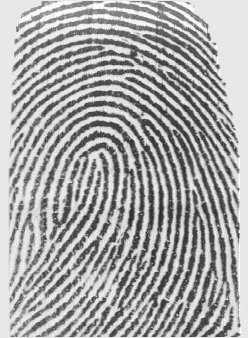
\includegraphics[scale=0.6]{Figures/example1_1}
         \caption{Example1\_1}
     \end{subfigure}%
     \quad
     \begin{subfigure}[t]{0.45\textwidth}
         \centering
         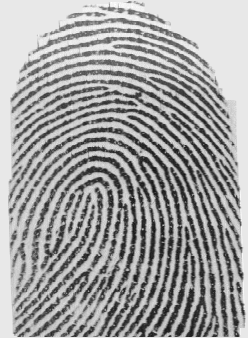
\includegraphics[scale=0.6]{Figures/example1_2}
         \caption{Example1\_2}
     \end{subfigure}
    \caption{Examples of fingerprints.}
    \label{fig:ex1a}
\end{figure}

As we can see, the pictures of the fingerprints have relatively high quality and its macro-singularities can be observed at first sight.

\subsection{ How many macro-singularities do you observe in each fingerprint?}

As we already know, macro-singularities can be loops, deltas or whorls.\\

In the previous figure we can observe a single loop in each of the fingerprints. No deltas or whorls have been found.

\subsection{ Mark the macro-singularities in the images (deltas and loops).}

We mark the previously mentioned loops using a red circle in Figure \ref{fig:ex1b}.

\begin{figure}[h!]
  \centering
       \begin{subfigure}[t]{0.45\textwidth}
         \centering
         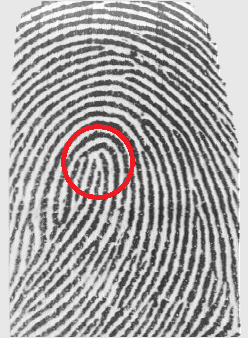
\includegraphics[scale=0.6]{Figures/example1_marked}
         \caption{Example1\_1 with a marked loop.}
     \end{subfigure}%
     \quad
     \begin{subfigure}[t]{0.45\textwidth}
         \centering
         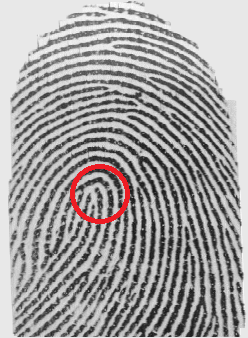
\includegraphics[scale=0.6]{Figures/example2_marked}
         \caption{Example1\_2 with a marked loop.}
     \end{subfigure}
    \caption{Marked loops.}
    \label{fig:ex1b}
\end{figure}

\section{Exercise 2}
\subsection{ Execute the provided code for Fingerprint Enhancement and paste the resulting image here}

We execute the Matlab script \inline{main.m} and stop it when the enhanced images are printed. The obtained enhanced fingerprints are shown in Figure \ref{fig:ex2a}.



\begin{figure}[h!]
  \centering
       \begin{subfigure}[t]{0.45\textwidth}
         \centering
         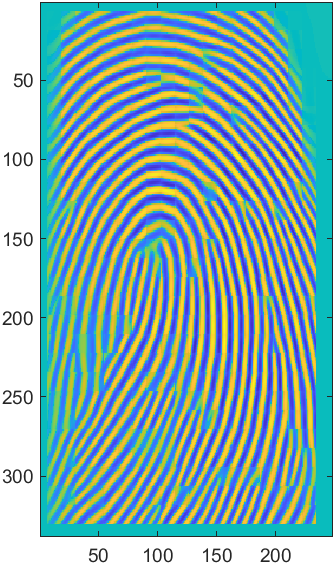
\includegraphics[scale=0.8]{Figures/Enhanced1}
         \caption{Example1\_1 enhanced.}
     \end{subfigure}%
     \quad
     \begin{subfigure}[t]{0.45\textwidth}
         \centering
         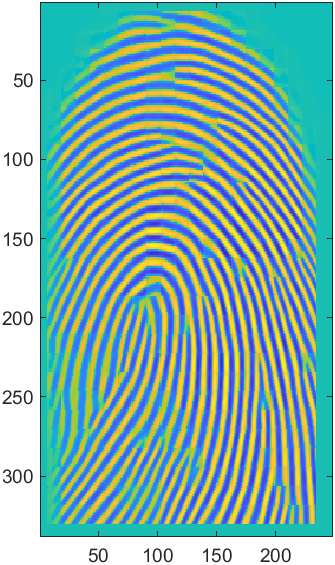
\includegraphics[scale=0.8]{Figures/Enhanced2}
         \caption{Example1\_2 enhanced.}
     \end{subfigure}
    \caption{Enhanced fingerprint examples.}
    \label{fig:ex2a}
\end{figure}


\subsection{ What differences do you observe with respect to the original fingerprints?}

The aim of the enhancement techniques is to improve the fingerprint image quality in order make the feature extraction task easier. Typically, we want to complete the ridge lines, deal with cuts or bruises on the finger or obtain a better separation between parallel ridges.

As we can see, the fingerprints in Figure \ref{fig:ex1a} had incomplete ridge lines at the bottom part of the image which have been completed in the enhancement in Figure \ref{fig:ex2a}.

Also, the image has been \emph{sharpened}, which means that now the contrast between the ridge lines and the \emph{white spaces} has been increased, making ridge lines easier to identify.


\section{Exercise 3}
\subsection{ Execute now the code for Quality Maps, and paste the resulting quality maps}

If we keep executing the \inline{main.m} script we obtain the following Quality Maps:



\begin{figure}[H]
  \centering
       \begin{subfigure}[t]{0.45\textwidth}
         \centering
         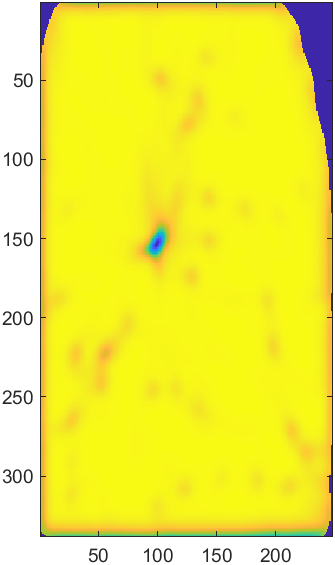
\includegraphics[scale=0.8]{Figures/QMap1}
         \caption{Quality Map of the first fingerprint.}
     \end{subfigure}%
     \quad
     \begin{subfigure}[t]{0.45\textwidth}
         \centering
         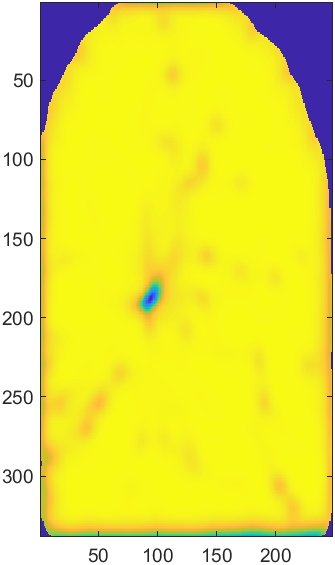
\includegraphics[scale=0.8]{Figures/QMap2}
         \caption{Quality Map of the second fingerprint.}
     \end{subfigure}
    \caption{Quality maps.}
    \label{fig:ex3a}
\end{figure}


\subsection{ What is the range of values for these quality maps?}

To obtain this quantities, we have added the following code to the main script: 

\begin{minted}{Matlab}
  min(relI1,[],'all')
  max(relI1,[],'all')
  
  min(relI2,[],'all')
  max(relI2,[],'all')
\end{minted}

This code shows that:

\begin{itemize}
  \item The minimum value for both Quality Maps is \(0.0\)
  \item The maximum value for the first fingerprint Quality Map is \(0.9991\)
  \item The maximum value for the second fingerprint Quality Map is \(0.9988\)
\end{itemize}

Thus, we can say that both Quality Maps have all its values in the range \([0,1]\).

\subsection{ What kind information (apart from the quality) can be inferred from such code?}

We examine the file \inline{testfin.m} to understand the result that we are obtaining.

If we read the first commented lines, we find that the function we applied returns
\begin{minted}{MatLab}
  % Returns:    newim - Ridge enhanced image.
  %             binim - Binary version of enhanced image.
  %             mask  - Ridge-like regions of the image
  %             reliability - 'Reliability' of orientation data  
\end{minted}
Considering this and the code of the \inline{main.m} file, what we just showed in Figure \ref{fig:ex3a} is the \textbf{reliabiltiy} of the orientation data, that is, how secure we are of the orientation of the ridge-lines in each point of the image. As we can see in the figure, we can say that we can not rely on the results outside the fingerprint, and that the algorithm has some problems in the zone where the loop is detected. This makes sense to us, since in the top of the loop the orientation of the ridge-line changes completely.  

We also find that the process followed to obtain the quality maps is:
\begin{enumerate}
\item Identify the ridge-like regions and normalise the image. We can see that different blocksizes and thresholds have been used but finally using \(blocksize=16\) and \(threshold = 0.1\) are the values used.
\item Determine the orientations of the found ridge-like regions.
\item Determine ridge frequency values across the image. Then, the median frequency is multiplied in the final mask that will be applied to the image (a comment says that the median frequency performed better than the actual frequency.)
\item Lastly, the filter is applied to enhance the patterns
\end{enumerate}




\section{Exercise 4}

\subsection{ Execute the code in order to show the Binarized Fingerprint and the Segmented Fingerprint. Apply different values of quality threshold (0.1, 0.3, 0.6, 0.9) and paste here the resulting images}

Let us first examine the code to see what we are doing in this section.

\begin{minted}{MatLab}
  %Binarized and Segmented Fingerprints
  threshold=0.1; %quality threshold
  figure;
  subplot(121)
  imagesc(binI1+mask1+(relI1>threshold)) 
  binI1(relI1<threshold)=0; 
  inv_binI1 = (binI1 == 0); 
\end{minted}

We can see that we stablish a threshold (which we are told to modify) and then plots an image that is an addition of the images:
\begin{itemize}
\item Enhanced binarized image
\item The mask that contains the ridge-like regions of the image (returned by testfin)
\item The reliability of the orientation, selecting the pixels where the reliability is above the selected threshold
\end{itemize}

The result of the code is shown in Figures \ref{fig:ex4-1st} and \ref{fig:ex4-2nd}.

\begin{figure}[h!]
  \centering
       \begin{subfigure}[t]{0.2\textwidth}
         \centering
         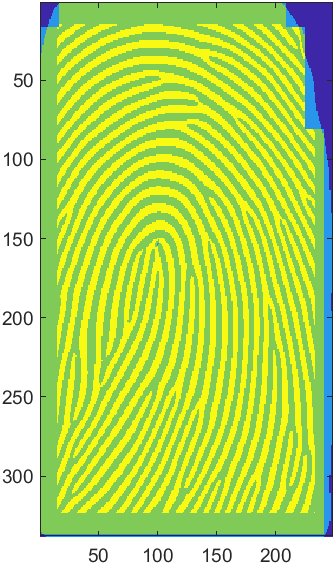
\includegraphics[scale=0.5]{Figures/E4-e1-0.1}
         \caption{\(0.1\)}
     \end{subfigure}%
     \quad
     \begin{subfigure}[t]{0.2\textwidth}
         \centering
         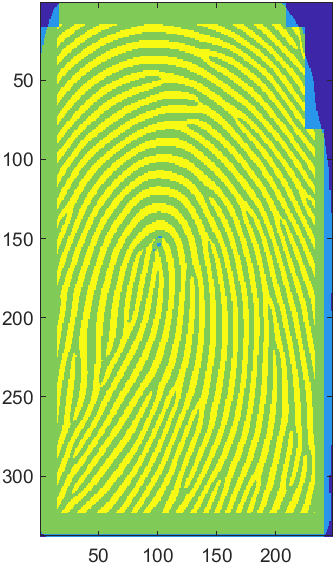
\includegraphics[scale=0.5]{Figures/E4-e1-0.3}
         \caption{\(0.3\)}
     \end{subfigure}
     \begin{subfigure}[t]{0.2\textwidth}
      \centering
      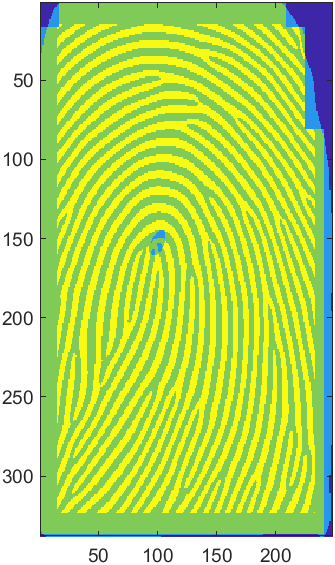
\includegraphics[scale=0.5]{Figures/E4-e1-0.6}
      \caption{\(0.6\)}
  \end{subfigure}%
  \quad
  \begin{subfigure}[t]{0.2\textwidth}
      \centering
      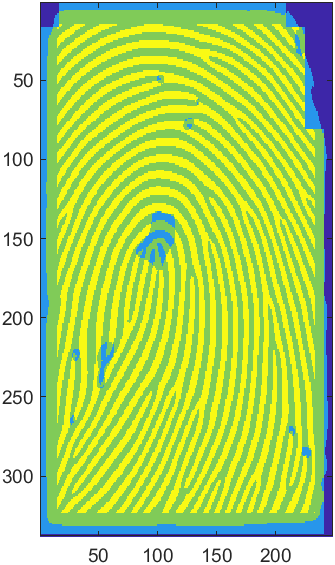
\includegraphics[scale=0.5]{Figures/E4-e1-0.9}
      \caption{\(0.9\)}
  \end{subfigure}
    \caption{Different thresholds for the first fingerprint example.}
    \label{fig:ex4-1st}
\end{figure}

\begin{figure}[h!]
  \centering
       \begin{subfigure}[t]{0.2\textwidth}
         \centering
         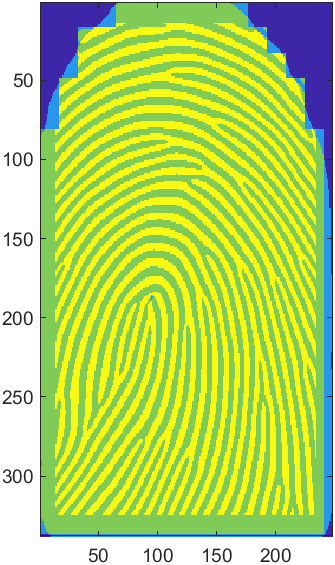
\includegraphics[scale=0.5]{Figures/E4-e2-0.1}
         \caption{\(0.1\)}
     \end{subfigure}%
     \quad
     \begin{subfigure}[t]{0.2\textwidth}
         \centering
         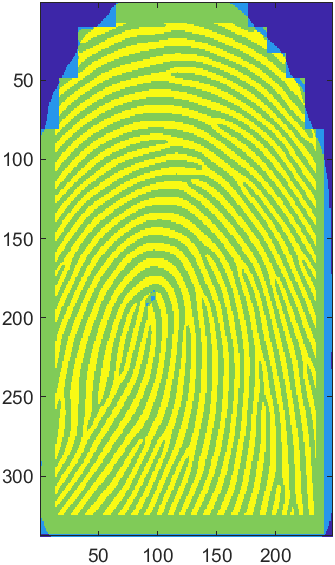
\includegraphics[scale=0.5]{Figures/E4-e2-0.3}
         \caption{\(0.3\)}
     \end{subfigure}
     \begin{subfigure}[t]{0.2\textwidth}
      \centering
      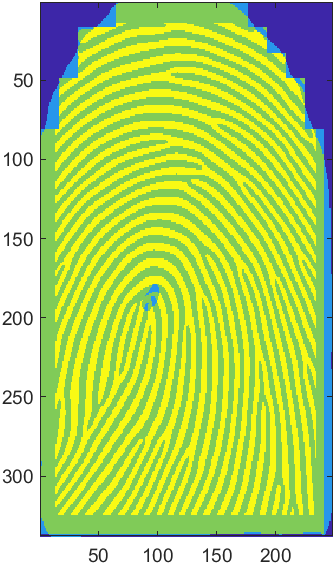
\includegraphics[scale=0.5]{Figures/E4-e2-0.6}
      \caption{\(0.6\)}
  \end{subfigure}%
  \quad
  \begin{subfigure}[t]{0.2\textwidth}
      \centering
      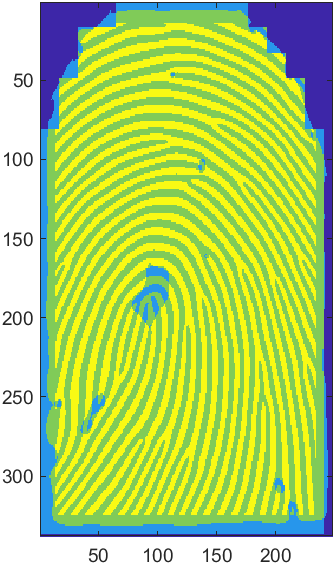
\includegraphics[scale=0.5]{Figures/E4-e2-0.9}
      \caption{\(0.9\)}
  \end{subfigure}
    \caption{Different thresholds for the second fingerprint example.}
    \label{fig:ex4-2nd}
\end{figure}

We can observe in both cases that, as the threshold is augmented, the reliability around the loops decreases and the yellow mask dissapear in both cases. This phenomenon also happens in other points that, until this point of the lab, we have not detected as important points.




\section{Exercise 5}
\subsection{ Execute the code for generating the Fingerprint Skeleton and the Minutiae Extractor. Paste the resulting images for the original values \(window=5\) and \(margin=5\). }






















\subsection{Search heuristically by looking at the images for the optimal values of parameters window and margin. Paste the resulting images with your optimal parameters and justify your decision.}




















\section{Exercise 6}

\subsection{ Execute the code corresponding to the Minutiae Validation for window=5 and margin=5.  Paste the resulting image including the minutiae extracted (red crosses) and validated (blue circles) of both fingerprints. }

















\subsection{ Execute the same code but with the optimal values of parameters window and margin. Paste the resulting image below. }


















\subsection{ Do you think it is a good idea to include the Minutiae Validation module? Justify your opinion. }




\section{Extra Exercise}
With all the previous exercises done correctly you can obtain a mark up to 7 points out of 10. 
Extra work: If you want to obtain a mark up to 10 points out of 10 you should complete the following:
In folder “/ddbb” you have 20 fingerprint images. 19 of them are labeled with the subject identity (e.g., H0001), and 1 is Unknown. Search for the identity of the Unknown fingerprint in the set of 19 labelled reference fingerprints. You can use the provided code “identification\_1\_19.m” as basis. Paste here the resulting ranked list of scores of the Unknown fingerprint with respect each one of the 19 reference fingerprints.





\end{document}
